\section{广度优先遍历}
\label{sec:graph-bfs}

给定一张图和一个起点，最基本的问题是：从起点出发能走到哪些顶点，走到每个顶点最少要经过几条边，又该沿哪条路线走。广度优先遍历按离起点的远近逐层访问顶点，一次就回答这三个问题，并且还能直接利用距离层数的奇偶性判定一张无向图是否为二部图。

\subsection{问题与思路}
\label{sec:graph-trav-bfs-problem}

输入是图$\mathcal G=(V,E)$的邻接表和一个起点$s\in V$。记$\operatorname{dist}(s,v)$为从$s$到$v$的路径所含的最少边数，有向图中路径沿弧的方向；$v$从$s$不可达时约定$\operatorname{dist}(s,v)=+\infty$。对每个顶点$v$，我们要知道它是否从$s$可达；若可达，$\operatorname{dist}(s,v)$是多少，以及一条恰好用$\operatorname{dist}(s,v)$条边从$s$走到$v$的路线。

按定义逐条检查路径是行不通的。从$s$到$v$的路径可能极多，而且路径越长，种类增长越快；即使只想知道最少边数，也不能把所有路径列出来再比较。

不枚举路径，可以按距离把顶点分层。距离为$0$的只有$s$自己，距离为$1$的恰好是$s$的邻居。距离为$2$的顶点不在前两层，却与第$1$层某个顶点相邻：从$s$走两条边能到达它，一条边到不了。一般地，前$k$层找全以后，第$k+1$层就是与第$k$层相邻、但还没出现过的顶点。于是从第$0$层开始，每次由当前层找出下一层，直到某一层为空。

一个顶点可能与上一层的多个顶点相邻，也可能与本层或更早的顶点相邻，所以它只能在第一次被找到时归入某一层，之后再遇到就跳过。找到它时顺手记下是从哪个顶点找到的，沿这些记录往回走，就能恢复一条路线。

\subsection{算法实现}
\label{sec:graph-trav-bfs-algorithm}

逐层推进不必真的维护一层层的列表，一个先进先出的队列就够了：先进入队列的顶点先展开，第$k$层的顶点全部展开完之前，第$k+1$层的顶点只在队尾排队。算法维护四项状态：
\begin{itemize}
  \item 发现标记：顶点是否已经被找到；
  \item 队列$Q$：已经发现、但邻居尚未检查的顶点；
  \item 边数距离$d(v)$：$v$被找到时所在的层号；
  \item \term{父指针}（parent pointer）$p(v)$：$v$是在展开哪个顶点时第一次被找到的。
\end{itemize}
初始时只有$s$被发现，$d(s)=0$，$p(s)$为空，$Q=[s]$；其余顶点未发现，$d(v)=+\infty$。

此后每一轮从队首取出一个顶点$u$，依次检查它的邻居。未发现的邻居$v$属于$u$的下一层：立即把它标记为已发现，写入$d(v)=d(u)+1$和$p(v)=u$，放到队尾。已发现的邻居则跳过。

队列变空时，从$s$可达的顶点都已找到。这种按层访问的过程称为广度优先遍历，也常称\term{广度优先搜索}（breadth-first search，BFS）。

\begin{algorithm}[广度优先遍历]
\label{alg:graph-trav-bfs}
输入：图$\mathcal G=(V,E)$的邻接表，起点$s\in V$。输出：距离$d(v)$与父指针$p(v)$，$v\in V$。
\begin{enumerate}
  \item 标记$s$为已发现，置$d(s)=0$、$p(s)$为空，令$Q=[s]$；其余顶点未发现，$d(v)=+\infty$。
  \item 当$Q$非空时，取出队首$u$，按邻接表依次读取$u$的邻居$v$（有向图只读出邻居$v\in N^+(u)$）。若$v$未发现，立即标记$v$为已发现，置$d(v)=d(u)+1$、$p(v)=u$，并把$v$放到队尾；若$v$已发现，跳过。
  \item 队列为空时停止。
\end{enumerate}
\end{algorithm}

要让每个顶点只在第一次被找到时归入某一层，必须在它入队时就做标记。两个已发现的顶点可能共享一个尚未发现的邻居；若等到出队时才标记，这个邻居会被两个顶点各放入队列一次，距离和父指针也可能被改写。入队即标记，每个顶点就至多入队一次。

\paragraph{执行过程}
在第~\ref{sec:graph-basic-concepts}节的贯穿四点图上，以$1$为起点，并约定按编号从小到大读取邻居。图~\ref{fig:graph-trav-bfs-queue}(b)逐行列出了每次出队后的队列。初始$Q=[1]$，此后四轮依次为：
\begin{itemize}
  \item 取出$1$：发现$2,3$，写入$d(2)=d(3)=1$、$p(2)=p(3)=1$，队列变为$[2,3]$。
  \item 取出$2$：邻居$1,3$都已发现，只有$4$是新的，写入$d(4)=2$、$p(4)=2$，队列变为$[3,4]$。
  \item 取出$3$：邻居$1,2,4$全部已发现，$4$不会第二次入队，队列变为$[4]$。
  \item 取出$4$：没有新顶点，队列为空，算法停止。
\end{itemize}
图~\ref{fig:graph-trav-bfs-queue}(a)把各顶点按$d$值分到三层，蓝色箭头就是父指针所指的边。

\begin{figure}[!htb]
  \centering
  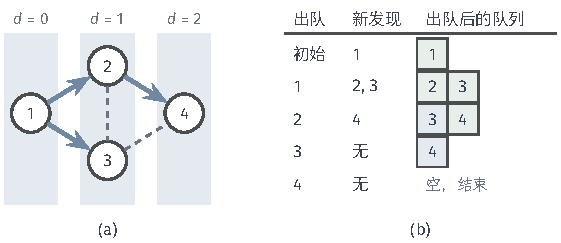
\includegraphics[width=94.963mm]{figures/01-basic-mathematics/04-graphs/tikz/c2-bfs-queue-trace/figure.pdf}
  \caption{贯穿四点图上从顶点$1$出发的广度优先遍历，邻居按编号递增读取。(a)顶点按边数距离$d$分为三层，蓝色箭头是父指针对应的边，虚线是检查过但没有带来新顶点的边。(b)每次出队后的队列，队首在左，绿色格子是这一步新入队的顶点；取出$3$时$4$已在队中，不再重复入队。}
  \label{fig:graph-trav-bfs-queue}
\end{figure}

\paragraph{路线的恢复}
要得到从$s$到已发现顶点$t$的路线，从$t$出发反复取父指针，直到回到$s$，再把得到的顶点序列反转。父指针总是指向更早发现的顶点，所以回溯不会绕圈，一定在有限步内回到$s$。

在上例中，$4$的父指针是$2$，$2$的父指针是$1$，反转后得到路线$1\to2\to4$，恰有$d(4)=2$条边。若$t$始终未被发现，即$d(t)=+\infty$，算法应报告$t$从$s$不可达，而不能输出任何路线。

路线并不唯一。若改为先读$3$再读$2$，取出$1$后队列为$[3,2]$，$4$在展开$3$时被发现，父指针变成$p(4)=3$，路线变成$1\to3\to4$。两条路线不同，边数却都是$2$：改变同层顶点的处理次序可能改变父指针，但下面的定理表明它不改变距离。

\subsection{算法分析}
\label{sec:graph-trav-bfs-correctness}

\paragraph{正确性}
算法只在顶点第一次被发现时写入$d(v)$，以后不再修改。正确性的关键在于，这个“第一次”恰好发生在最短的距离上。

\begin{theorem}[广度优先遍历的距离]
\label{thm:graph-trav-bfs-distance}
设对有限图$\mathcal G$和起点$s$执行算法~\ref{alg:graph-trav-bfs}。则对每个顶点$v$，$d(v)=\operatorname{dist}(s,v)$；当$v$可达时，沿父指针从$v$回到$s$的路线恰有$d(v)$条边。
\end{theorem}

\begin{proof}
先说明$d(v)$不会小于真实距离。若$d(v)$有限且$v\neq s$，则$d(p(v))=d(v)-1$，沿父指针每退一步距离减一，$d(v)$步后回到$s$。反转这串顶点就得到一条从$s$到$v$、恰有$d(v)$条边的路线，所以$d(v)\geq\operatorname{dist}(s,v)$。

再说明队列中的距离值有一个固定的形状：从队首到队尾不减，且最大值与最小值至多相差$1$。初始队列只有$s$，满足这一点。设某时刻队列中的值为若干个$k$后接若干个$k+1$，取出的队首$u$有$d(u)=k$，新加入的顶点距离都是$k+1$，并放在队尾，形状仍然保持。由此可知，顶点出队时的距离值按时间不减。

最后对$\delta=\operatorname{dist}(s,v)$归纳，证明有限距离的顶点都会被发现且$d(v)\leq\delta$。$\delta=0$时$v=s$。设$\delta\geq1$，并设距离小于$\delta$的顶点都已满足结论。取一条从$s$到$v$的最短路径，记其倒数第二个顶点为$x$，则$\operatorname{dist}(s,x)=\delta-1$，由归纳假设$x$被发现且$d(x)=\delta-1$。

$x$入过队，就一定在某一时刻出队并检查邻居$v$。若此时$v$尚未发现，就得到
\[
d(v)=d(x)+1=\delta;
\]
若$v$已经被发现，则发现它的顶点$u$出队不晚于$x$，按上一段的单调性$d(u)\leq d(x)$，于是
\[
d(v)=d(u)+1\leq d(x)+1=\delta.
\]

两个方向合起来得到$d(v)=\operatorname{dist}(s,v)$。不可达的顶点没有任何从$s$出发的路线，第一段说明它不可能得到有限的$d$值。
\end{proof}

证明第二段的队列形状把“逐层推进”变成了可以检验的事实：处理第$k$层时只会首次发现第$k+1$层的顶点，而它们全部排在第$k$层之后。最短路径上的倒数第二个顶点$x$比$v$少一层，一定先被展开，所以$v$不会拖到更远的层才被发现。

\paragraph{复杂度}
以邻接表存储时，每个顶点至多入队、出队各一次，出队时把它的邻接表读一遍，因此每条邻接记录只被检查常数次。无向图的邻接记录共$2m$条，有向图的出邻接记录共$m$条，总时间为$O(n+m)$。发现标记、距离、父指针和队列各占$O(n)$额外空间。

这一结论依赖“列出邻居的代价与度数成正比”。若改用邻接矩阵，找出一个顶点的邻居要扫描一整行，$n$个顶点共扫描$n^2$个位置，时间变为$O(n^2)$；对稀疏图，这比$O(n+m)$大得多。

\paragraph{适用范围}
广度优先遍历把每条边都算作一步，而边上带有长度时，边数最少的路线不一定总长度最小。图~\ref{fig:graph-trav-bfs-weighted}中，从$s$直接到$t$只需一条边，广度优先遍历就用这条边记录$t$，但它的长度是$5$；经过$a$的路线多走一条边，总长度却只有$1+1=2$。所以广度优先遍历适用于所有边长相等且非负时的最短路问题。一般边长下的最短路需要比较累计长度，留到第~\ref{sec:graph-shortest-paths}章。

\begin{figure}[!htb]
  \centering
  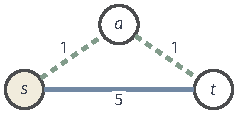
\includegraphics[scale=1]{figures/01-basic-mathematics/04-graphs/tikz/c2-bfs-weighted-counterexample/figure.pdf}
  \caption{带权反例。边旁数字是长度。广度优先遍历从$s$出发时经直接边一步发现$t$（蓝色），这条路线总长$5$；绿色虚线路线$s\text{--}a\text{--}t$多一条边，总长只有$2$。广度优先遍历最小化的是边数，不是总长度。}
  \label{fig:graph-trav-bfs-weighted}
\end{figure}

一次广度优先遍历也只覆盖从$s$可达的部分。遍历结束时距离仍为$+\infty$的顶点没有被访问，不能据此断言它们是孤立点，它们之间可能有很多边。要给全图的每个顶点划分连通分量，需要在外层不断换新的起点重新启动，这是第~\ref{sec:graph-connectivity-computation}节的内容。

\subsection{多源广度优先遍历}
\label{sec:graph-trav-multi-source-bfs}

有时关心的不是离某一个起点多远，而是离一组起点中最近的那个多远。例如在网格上放置若干个种子，问每个格子离最近的种子几步。给定起点集合$S\subseteq V$，要求的是
\begin{equation}
\operatorname{dist}(S,v)=\min_{s\in S}\operatorname{dist}(s,v),
\label{eq:graph-trav-multi-source-dist}
\end{equation}
空集上的最小值约定为$+\infty$；同时还想知道$v$离哪个起点最近。

既然只关心最近的起点，就把$S$中的所有顶点一起当作第$0$层，从这一层开始逐层推进。实现上只改初始化：$S$中所有顶点都标记为已发现、距离为$0$、父指针为空，并按任意次序全部放入队列；此后的更新与算法~\ref{alg:graph-trav-bfs}完全相同。这称为\term{多源广度优先遍历}（multi-source breadth-first search）。

它的正确性可以归结到单源情形。设想添加一个新顶点$s^*$，从它向$S$中每个顶点连一条边（有向图中连弧$s^*\to s$）。因为从$s^*$出发的路线第一步必然进入$S$，新图中任一原顶点$v$满足
\[
\operatorname{dist}(s^*,v)=1+\operatorname{dist}(S,v).
\]
从$s^*$做普通广度优先遍历，第一次出队就把$S$中所有顶点以距离$1$放入队列，此后的过程与多源版本完全相同，只是所有距离多了$1$。

把定理~\ref{thm:graph-trav-bfs-distance}用于新图，再减去多出的$1$，可知多源版本输出$\operatorname{dist}(S,v)$。沿父指针回溯会停在某个起点上，回溯路线恰有$\operatorname{dist}(S,v)$条边，所以这个起点就是离$v$最近的起点之一。

图~\ref{fig:graph-trav-multi-source}是一个$3\times5$网格，相邻格子以上下左右相连，中间一个格子不属于图。两个起点放在左上角和右下角，每个格子中的数字是它到较近起点的边数。例如第一行第四个格子离左上角$3$步、离右下角也是$3$步，记为$3$，两个起点都是它的最近起点；第一行最右的格子离右下角只有$2$步，记为$2$。若只从左上角出发，右下角的格子距离为$6$。

\begin{figure}[!htb]
  \centering
  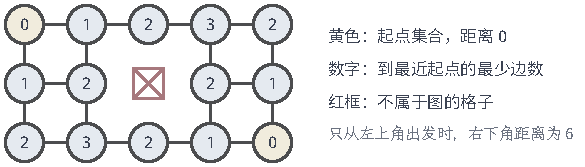
\includegraphics[width=99.0mm]{figures/01-basic-mathematics/04-graphs/tikz/c2-multi-source-bfs/figure.pdf}
  \caption{$3\times5$网格上的多源广度优先遍历。网格以上下左右相邻连边，红框格子不属于图；两个黄色起点同时作为第$0$层。每个顶点中的数字是到较近起点的最少边数，所有距离由一次遍历得到。}
  \label{fig:graph-trav-multi-source}
\end{figure}

对每个起点各做一次广度优先遍历，回答的是另一个问题：它得到$|S|$组距离，能说出$v$到每个起点各有多远，需要$O(|S|(n+m))$时间。多源遍历只给出到最近起点的距离及对应的起点，一次只需$O(n+m)$时间。若$S$为空，队列一开始就为空，所有顶点保持未发现，与$\operatorname{dist}(\varnothing,v)=+\infty$的约定一致。

\paragraph{来源标签的同步传播}
逐个回溯父指针才能知道来源，每次要花与距离成正比的时间。若需要全部顶点的最近来源，可以让来源随发现一起传下去。为此再维护一个数组$\operatorname{src}(\cdot)$，它的初始化与更新规则是：
\begin{itemize}
  \item 初始化时，对每个$s\in S$置$\operatorname{src}(s)=s$；
  \item 展开$u$时每发现一个新顶点$v$，除写入$d(v)$和$p(v)$外，再置$\operatorname{src}(v)=\operatorname{src}(u)$。
\end{itemize}

由于$p(v)=u$，按父指针归纳可知$\operatorname{src}(v)$就是从$v$回溯父指针到达的起点，所以它是$v$的一个最近来源。离两个起点一样近的顶点（例如上面网格第一行第四个格子）只记录先发现它的那一个；需要全部最近来源时，要在距离相等的情形下另行合并记录。

\subsection{二部图的判定}
\label{sec:graph-bfs-bipartite}

第~\ref{sec:graph-bipartite-graphs}小节的定理~\ref{thm:graph-bipartite-odd-cycle}证明，一张无向图是二部图当且仅当它不含奇环，而充分性的证明正是按每个顶点到基准起点的最少边数$\delta(v)$的奇偶性将顶点集划分为两部分。广度优先遍历算出的层数$d(v)=\operatorname{dist}(s,v)$恰好就是最少边数，因此把广度优先遍历的层次划分直接用作二染色，就能在$O(n+m)$时间内判定任意无向图是否为二部图，并在不是二部图时提取出一个可逐边核对的奇环。

具体而言，在某个连通分量中任选起点$s$，令第$0$层的$s$染颜色$c(s)=0$（归入$X$）。要使每条边两端异色，第$1$层的所有顶点都必须染$1$（归入$Y$），第$2$层的顶点又必须染$0$（归入$X$），一般地，第$k$层顶点$v$在首次被发现时赋予颜色$c(v)=d(v)\bmod 2=(c(u)+1)\bmod 2$，其中$u=p(v)$是发现它的上一层顶点。如果原图有多个连通分量，只需在外层依次扫描全部顶点，每遇到一个尚未着色的顶点就以它为起点启动一次广度优先遍历。

在展开队首顶点$u$、检查它的邻居$v$时，若$v$尚未发现，按$c(v)=1-c(u)$赋色入队，边$\{u,v\}$作为生成树上的父边天然满足两端异色。若$v$已被发现，则边$\{u,v\}$不是新的树边，此时比较$c(u)$与$c(v)$：当$c(v)\neq c(u)$时，说明$u$与$v$所处层数的奇偶性相反，这条边跨越$X$与$Y$，不破坏二部划分；当$c(v)=c(u)$时，说明$d(u)$与$d(v)$奇偶性相同，同一层（或同奇偶层）的两个顶点之间出现了直接连边，二部划分在此处发生冲突。一旦发现这样的同色边$\{u,v\}$，分别从$u$和$v$沿父指针$p(\cdot)$向起点回溯，找出它们在广度优先树上的最近公共祖先$w$；从$w$沿树边到$u$的路径（长$d(u)-d(w)$）、边$\{u,v\}$以及从$v$沿父指针回到$w$的路径（长$d(v)-d(w)$）除公共顶点$w$外互不相交，合起来恰好围成一个长度为$(d(u)-d(w))+(d(v)-d(w))+1$的简单奇环。

\begin{algorithm}[基于BFS的二部图判定与奇环提取]
\label{alg:graph-trav-bfs-bipartite}
输入：无向图$\mathcal G=(V,E)$的邻接表。输出：二部划分$(X,Y)$，或一个奇环$C$。
\begin{enumerate}
  \item 初始化所有顶点$v\in V$未发现，$d(v)=+\infty$，父指针$p(v)$为空，颜色$c(v)=-1$。
  \item 依次扫描$s\in V$；若$s$已发现则跳过，否则标记$s$已发现，置$d(s)=0$、$c(s)=0$，令队列$Q=[s]$。
  \item 当$Q$非空时，取出队首$u$，依次读取$u$的邻居$v\in N(u)$：若$v$未发现，标记$v$已发现，置$d(v)=d(u)+1$、$p(v)=u$、$c(v)=1-c(u)$，并把$v$放到队尾；若$v$已发现且$c(v)=c(u)$，从$u$和$v$沿父指针$p(\cdot)$回溯至最近公共祖先$w$，将$w\leadsto u$的树路径、边$\{u,v\}$与$v\leadsto w$的树路径拼接为奇环$C$，返回“非二部图”及奇环$C$。
  \item 全部顶点扫描完毕且未发生同色冲突时，输出二部划分$X=\{v\in V:c(v)=0\}$与$Y=\{v\in V:c(v)=1\}$。
\end{enumerate}
\end{algorithm}

\paragraph{执行过程与奇环恢复}
以贯穿四点图\eqref{eq:graph-conn-running-graph}与删去边$\{2,3\}$所得的四元环$\mathcal G-\{2,3\}$对照演示算法~\ref{alg:graph-trav-bfs-bipartite}。在贯穿图上从$s=1$启动：顶点$1$置$d(1)=0$、$c(1)=0$，队列$Q=[1]$；取出$1$后发现邻居$2,3$，写入$d(2)=d(3)=1$、$p(2)=p(3)=1$、$c(2)=c(3)=1$，队列变为$[2,3]$；接着取出$2$，检查邻居$1,3,4$，其中$1$已发现且$c(1)=0\neq c(2)$，而读到邻居$3$时发现$3$已着色且$c(3)=1=c(2)$。算法立即在同色边$\{2,3\}$处停下，从$2$和$3$沿父指针$p(2)=1$、$p(3)=1$回溯一步即汇合于最近公共祖先$w=1$，拼出长度为$3$的奇环$C=(1,2,3,1)$。

在删去$\{2,3\}$后的四元环上，同样从$s=1$启动：取出$1$后$2,3$染颜色$1$，队列为$[2,3]$；取出$2$时邻居只有$1$和$4$，$1$颜色为$0\neq c(2)$，未发现的$4$写入$d(4)=2$、$p(4)=2$、$c(4)=0$并入队；取出$3$时邻居$1$和$4$的颜色都是$0\neq c(3)$；取出$4$时邻居$2$和$3$的颜色都是$1\neq c(4)$。队列变空而没有任何边触发同色冲突，算法输出二部划分$X=\{1,4\}$、$Y=\{2,3\}$。

\paragraph{正确性与复杂度}
若算法在步骤4正常结束，则每条边$\{u,v\}\in E$在端点$u$出队时都被检查过且满足$c(v)\neq c(u)$，因此$X$与$Y$内部都没有边，$(X,Y)$确为合法的二部划分；若算法在步骤3因$c(v)=c(u)$停下，则$u$与$v$属于同一连通分量的广度优先树，必有公共祖先，最近公共祖先$w$到$u$和$v$的两条树路径除$w$外无公共顶点，且由于$d(u)\equiv c(u)=c(v)\equiv d(v)\pmod 2$，围成的环长$(d(u)-d(w))+(d(v)-d(w))+1$必为奇数，给出了定理~\ref{thm:graph-bipartite-odd-cycle}中不可二部化的直接证据。外层扫描与广度优先遍历合计访问每个顶点和每条边常数次，发现同色边后沿父指针回溯至多走$O(n)$步，故总时间复杂度为$O(n+m)$，额外空间为$O(n)$。
